\begin{figure}[ht!]
    \centering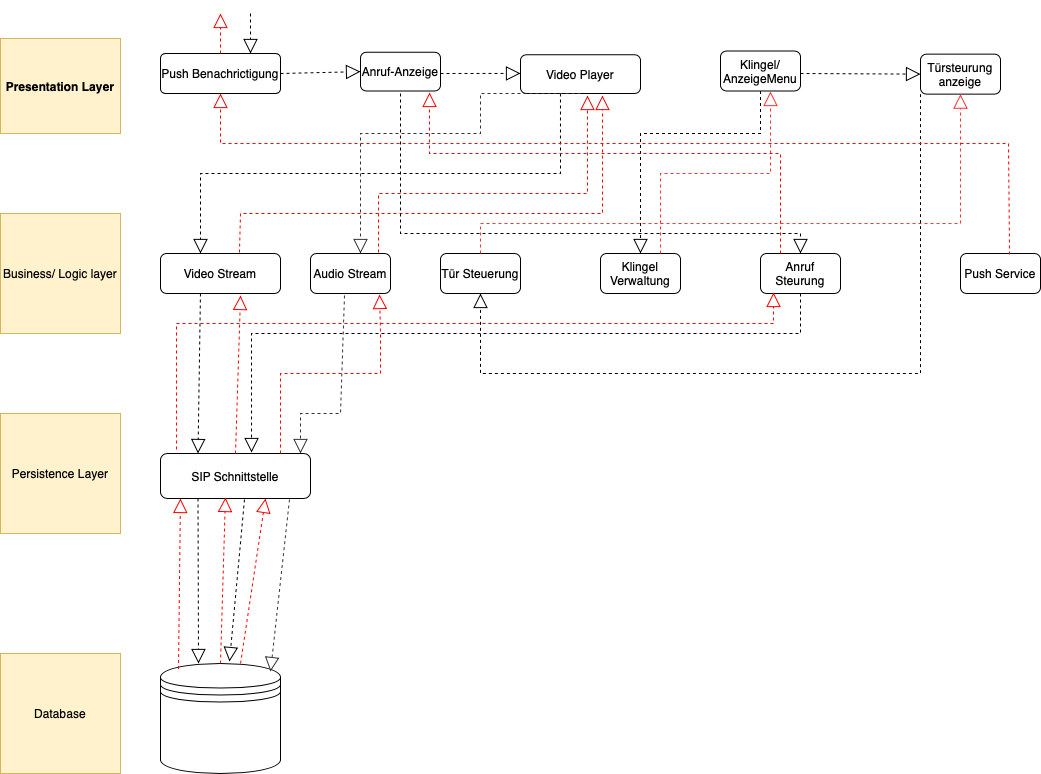
\includegraphics[width=\paperwidth/2]{../assets/img/layered-architecture-pattern.drawio}
    \caption{Architektur als Schichtenmodell}
    \label{fig:schichtenmodell}
\end{figure}
Wenn eine Push-Nachricht, wie in Abbildung~\ref{fig:schichtenmodell} dargestellt, auf der Anrufanzeige angezeigt wird und ein Klick/Auswahl zur Annahme eines Anrufs erfolgt, wird eine Nachricht an die Anrufsteurung gesendet, die sich mit der SIP-Schnittstelle und weiter mit der Datenbank verbindet, um die Anrufdaten (Datum und Uhrzeit) in der Datenbank zu speichern.
Die Anrufsteurung sendet eine entsprechende Meldung an die Anrufanzeige und eine entsprechende Meldung wird angezeigt, d.h.\ Annehmen oder Ablehnen.


Wird der Anruf angenommen, wird eine Nachricht an den Videostream in der Logikschicht gesendet, der sich mit der SIP Scnittstelle und weiter zur Datenbank verbindet, um die Video- und Audiodaten zu speichern.
Das Video- und Audiostreaming beginnt und der Videoplayer wird gestartet.


Das Klingel- und Anzeigemenu spiegelt alles wider, was in der KlingelVerwaltung gemacht wurde.
Auf der anderen Seite spiegelt die Türsteurung-Anzeige die Entscheidungen der Türsteurung in der Logikschicht wider.
